\chapter{Graphing Polynomials}

In using polynomials to solve real-world problems, it is often handy
to know what the graph of the polynomial looks like. You have many of
the tools you need to start to sketch out the the graphs:
\begin{itemize}
\item To find where the graph crosses the y-axis, you can evaluate the polynomial at $x = 0$.
\item To find where the graph crosses the x-axis, you can find the roots of the polynomial.
\item To find the level spots on the graph (often the top of a hump or the bottom of a dip), you can take the derivative of the polynomial (which is a polynomial), and find the roots of that.
\end{itemize}\index{polynomial!graphing}

\textit{FIXME: Diagram of those things}

For example, if you wanted to graph the polynomial $f(x) = -x^3 -x^2 +
6x$, you might plug in a few values that are easy to compute:
\begin{itemize}
\item $f(-2) = -8$
\item $f(-1) = -6$
\item $f(0) = 0$
\item $f(1) = 4$
\item $f(2) = 0$ 
\end{itemize}

So, right away, we know two roots: $x = 0$ and $x = 2$. Are there
others? We won't know until we factor the polynomial:
\begin{multline*}
  -x^3 -x^2 + 6x \\
  = (-1x)(x^2 + x - 6) \\
  = (-1x)(x + 3)(x - 2)
\end{multline*}
So, yes, there is a third root: $x = -3$

What about the level spots? $f'(x) = -3x^2 - 2x + 6$. Where is that zero?
\begin{multline*}
  -3x^2 -2x + 6 = 0 \\
  x^2 + \frac{2}{3}x - 2 = 0
\end{multline*}
We have a formula for quadratics like this:
\begin{multline*}
  x = -\frac{b}{2} \pm \frac{\sqrt{b^2 - 4c}}{2} \\
  = -\frac{\frac{2}{3}}{2} \pm \frac{\sqrt{\left(\frac{2}{3}\right)^2 - 4(-2)}}{2} \\
  = -\frac{1}{3} \pm \frac{\sqrt{\frac{4}{9} + 8}}{2} \\
  = -\frac{1}{3} \pm \frac{\sqrt{\frac{85}{9}}}{2} \\
  = -\frac{1}{3} \pm \frac{\sqrt{85}}{6} \\
  \approx 1.20 \text{ and } -1.87 
\end{multline*}

Now, you might plug those numbers in:
\begin{itemize}
\item $f(1.2) \approx 4.0 $
\item $f(-1.87) \approx -8.2$
\end{itemize}

\section{Leading term in graphing}

There is one more trick you need before you can draw a good graph of a
polynomial. As you go father and farther to the left and right, where
does the function go? In other words, does the graph go up on both ends
(like a smile)? Or does it go down on both ends (like a frown)? Or
does the negative end go down (frowny) while the positive end go up
(smiley)? Or does the negative go up (smiley) and the positive end go
down (frowny)?

Assuming the polynomial is not constant, there are only those four
possibilties. It is determined entirely by the leading term of the
polynomial.  If the degree of the leading term is even, both ends go
in the same direction (both are smiley or both are frowny).  If the
coefficient of the leading term is positive, the positive end is
smiley.

The graph we are working on has a leading term of $-1x^3$. The degree is odd, thus the ends go in different directions. The coefficient is negative, so the positive end points down.  Now, you can draw the graph, which should look something like this:
\begin{figure}[htbp]
    \centering
    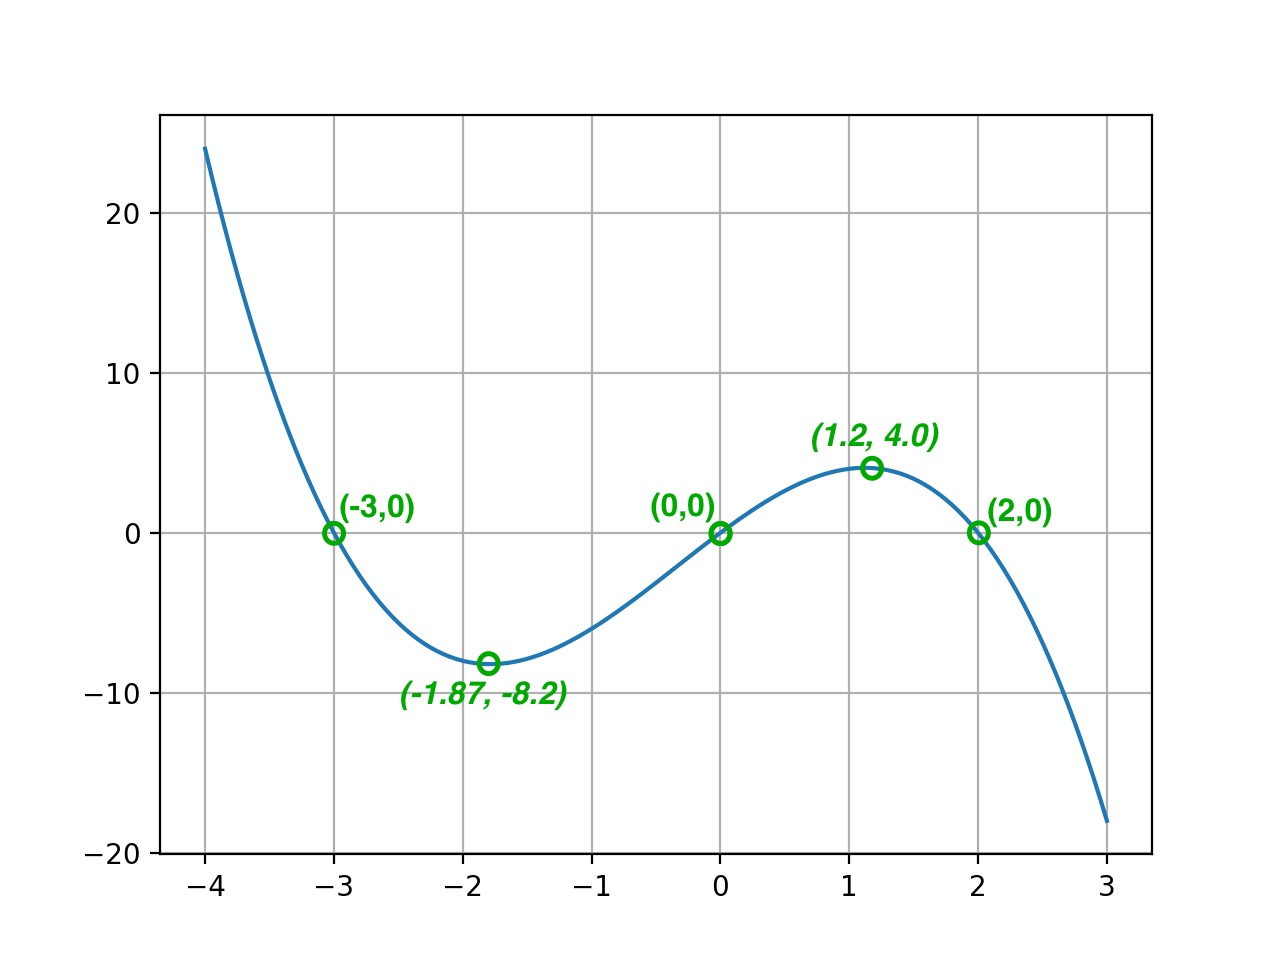
\includegraphics[width=\textwidth]{annotated_graph.png}
    \caption{A graph with roots and significant points.}
    \label{fig:annotated_graph}
\end{figure}
